\documentclass[12pt, journal, onecolumn]{IEEEtran}
\raggedbottom
%
\usepackage{instructivo}  % Commands for multiple choice
\graphicspath{{./}{./fig/}}

\usepackage[natbib=true,style=trad-unsrt,backend=biber]{biblatex}

\addbibresource{literatura.bib}
\usepackage{multirow}
\usepackage{graphicx}
\usepackage{array}
\usepackage{float}
\usepackage{capt-of}
\usepackage{hyperref}
\newcolumntype{C}{>{\centering\arraybackslash}X}
% correct bad hyphenation here
\hyphenation{op-tical net-works semi-conduc-tor}


\begin{document}
	%
	% paper title
	% Titles are generally capitalized except for words such as a, an, and, as,
	% at, but, by, for, in, nor, of, on, or, the, to and up, which are usually
	% not capitalized unless they are the first or last word of the title.
	% Linebreaks \\ can be used within to get better formatting as desired.
	% Do not put math or special symbols in the title.
\title{Proyecto: Semáforo Vehicular y Peatonal}
	
	
\author{Gerald~David~Blanco-Sáenz,~\IEEEmembership{Estudiante,~ITCR},~Melanie~Espinoza-Hernandez,~\IEEEmembership{Estudiante,~ITCR},~Nayshell~Freckleton-White,~\IEEEmembership{Estudiante,~ITCR} 
	y~Pablo~Cabrera-Montealegre,~\IEEEmembership{Estudiante,~ITCR}}
	
	
	% The paper headers
\markboth{EL3215 Laboratorio de Electrónica Analógica, IS2026}%
{EL3215 Laboratorio de Electrónica Analógica}
	
	
	% make the title area
\maketitle
	
\begin{abstract}
		Se propone el diseño de un sistema de semáforo vehicular y peatonal, cuyo objetivo principal es simular un cruce vehicular completo mediante la gestión del flujo de tránsito y la interacción a través de solicitudes peatonales. El sistema incorpora señalización visual (rojo, amarillo, verde) y auditiva, control de tiempos regresivos mediante displays, y una etapa de conversión de energía de corriente alterna (CA) a corriente directa (CD). En este primer avance, se documenta exclusivamente la etapa de alimentación del circuito, la cual es responsable de proveer los niveles de tensión regulados adecuados para el funcionamiento de las etapas analógicas y digitales posteriores.
\end{abstract}
	
\section{Introducción}
	Los sistemas de control de tráfico son fundamentales para la regulación segura y eficiente de la movilidad vehicular y peatonal en entornos urbanos. Estos sistemas integran elementos de temporización, señalización visual y auditiva, así como mecanismos de interacción con los usuarios. En el contexto de la ingeniería electrónica, el diseño de un sistema de semáforo permite aplicar conceptos relacionados con la generación de señales, temporización, control lógico, visualización de información y procesamiento de señales de audio. Además, representa un ejemplo claro de integración de subsistemas analógicos y digitales en una aplicación real. \\
	
	Este proyecto se enfoca en el diseño e implementación de un sistema completo de semáforo vehicular y peatonal, utilizando componentes electrónicos discretos y circuitos digitales básicos, evitando el uso de dispositivos programables de acuerdo con las especificaciones. El objetivo principal de este primer documento es presentar la propuesta de diseño de cada etapa del sistema, detallando sus componentes y la justificación de las decisiones de diseño.
	
	\section{Objetivos}
	\subsection{Objetivo General}
	Introducir al estudiante ante un problema de ingeniería en donde requiera poner en práctica las habilidades y conceptos adquiridos en el uso de las herramientas de simulación, equipos de medición, prototipado y ensamble de circuitos eléctricos transistorizados por medio de circuitos impresos.
	
	\subsection{Objetivos Específicos}
	\begin{itemize}
		\item Introducir al estudiante en el diseño de ingeniería bajo el establecimiento de una solución a un problema planteado.
		\item Utilizar herramientas de simulación en la etapa de diseño de sistemas electrónicos que integren etapas analógicas y digitales.
		\item Desarrollar habilidades de implementación de sistemas electrónicos bajo el apoyo de equipo especializado para mediciones.
		\item Adquirir conocimiento y habilidades necesarias para el diseño e implementación de circuitos impresos o PCB para ensamble de circuitos eléctricos.
		\item Fomentar las habilidades requeridas para el trabajo en equipo en proyectos de ingeniería.
	\end{itemize}
	
	\section{\textbf{Alimentación}}
	\subsection{Descripción}
	Para el funcionamiento del semáforo eléctrico y sus respectivos sistemas lógicos, se requiere una fuente de alimentación que convierta la energía proveniente de la red eléctrica de 120\,$\text{V}_{\text{rms}}$ a 60\,Hz en niveles de tensión de corriente directa (CD) regulados y ajustados. Estos voltajes son vitales para cumplir con las condiciones de operación de las compuertas lógicas, los circuitos de temporización y las etapas de potencia para la señalización visual y acústica.\\
	
	El circuito convertidor de CA a CD incluye los siguientes componentes principales: un transformador reductor, un puente rectificador de onda completa, capacitores de filtrado y reguladores de voltaje lineal. Estos elementos actúan en conjunto para entregar las tensiones estables que requiere el resto del sistema, protegiendo los componentes de variaciones indeseadas.
	
	\subsection{Diagrama del circuito}
	\begin{figure}[h]
		\centering
		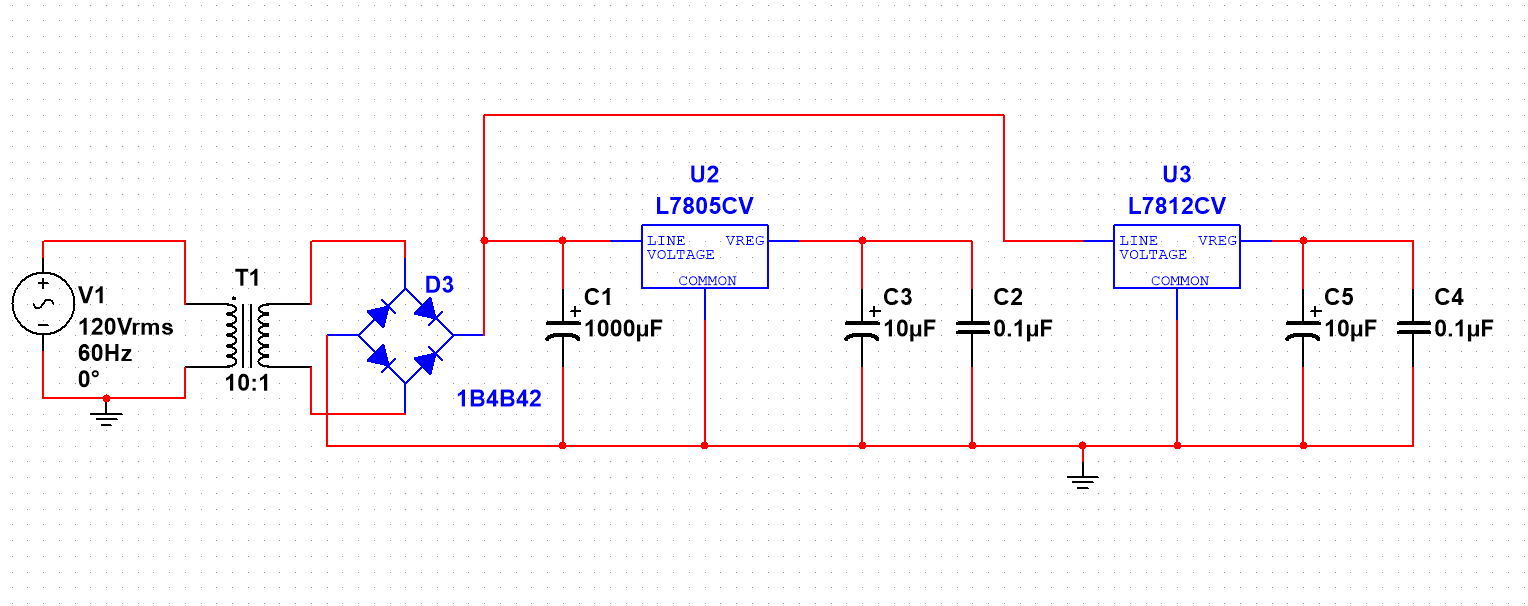
\includegraphics[width=0.7\textwidth]{diagrama_alimentacion.png}
		\caption{Diagrama del circuito de Alimentación.}
		\label{fig:alimentacion}
	\end{figure}
	
	\subsection{Justificación de diseño}
	El diseño del circuito de alimentación de la Fig. \ref{fig:alimentacion} se fundamenta en la necesidad de convertir los 120\,$\text{V}_{\text{rms}}$ de corriente alterna (CA) a voltajes de corriente directa (CD) regulados estables, habitualmente de 5\,V para los componentes de lógica digital (TTL/CMOS), y otros voltajes mayores (como 12\,V) si así lo requieren la amplificación de la señal acústica o los arreglos de LEDs de alta luminosidad.\\
	
	Inicialmente, el transformador reductor disminuye el voltaje de entrada a un nivel seguro y apto para su manipulación. Luego, el puente rectificador de diodos convierte la señal alterna en una señal pulsante en una sola dirección. Para disminuir el rizado de esta señal, se incorporan capacitores de gran valor en capacitancia que filtran las oscilaciones y otorgan una primera etapa de estabilización a la señal.\\
	
	Finalmente, los reguladores de voltaje integrados (como los de la familia 78XX) proporcionan una salida continua y fija, absorbiendo las variaciones en el consumo de corriente al encender diferentes estados del semáforo. Se agregan capacitores de desacople adicionales en los terminales de entrada y salida de estos reguladores para estabilizar la respuesta transitoria del dispositivo y atenuar posibles ruidos de alta frecuencia introducidos por la conmutación lógica, garantizando así un desempeño ininterrumpido en todo el circuito de control de tráfico.\\

\newpage

\section{\textbf{Máquina de estados}}
\subsection{Descripción}
Esta subsección describe el circuito encargado de controlar la lógica completa del semáforo vehicular y peatonal, incluyendo la generación de estados, temporización, control de transición y activación de las señales luminosas. El circuito implementa una máquina de estados síncrona basada en lógica digital discreta, utilizando compuertas lógicas, contadores y temporizadores, cumpliendo con las especificaciones establecidas para el proyecto de semáforo vehicular y peatonal.\\

La FSM consta de cuatro estados codificados mediante dos bits, los cuales son almacenados en dos flip-flops JK CD4027 sincronizados por una señal de reloj generada con un temporizador 555. Cada estado representa una etapa específica del funcionamiento del semáforo peatonal y vehicular, permitiendo controlar tanto las luces como las señales sonoras del sistema.\\

	\begin{figure}[H]
		\centering
		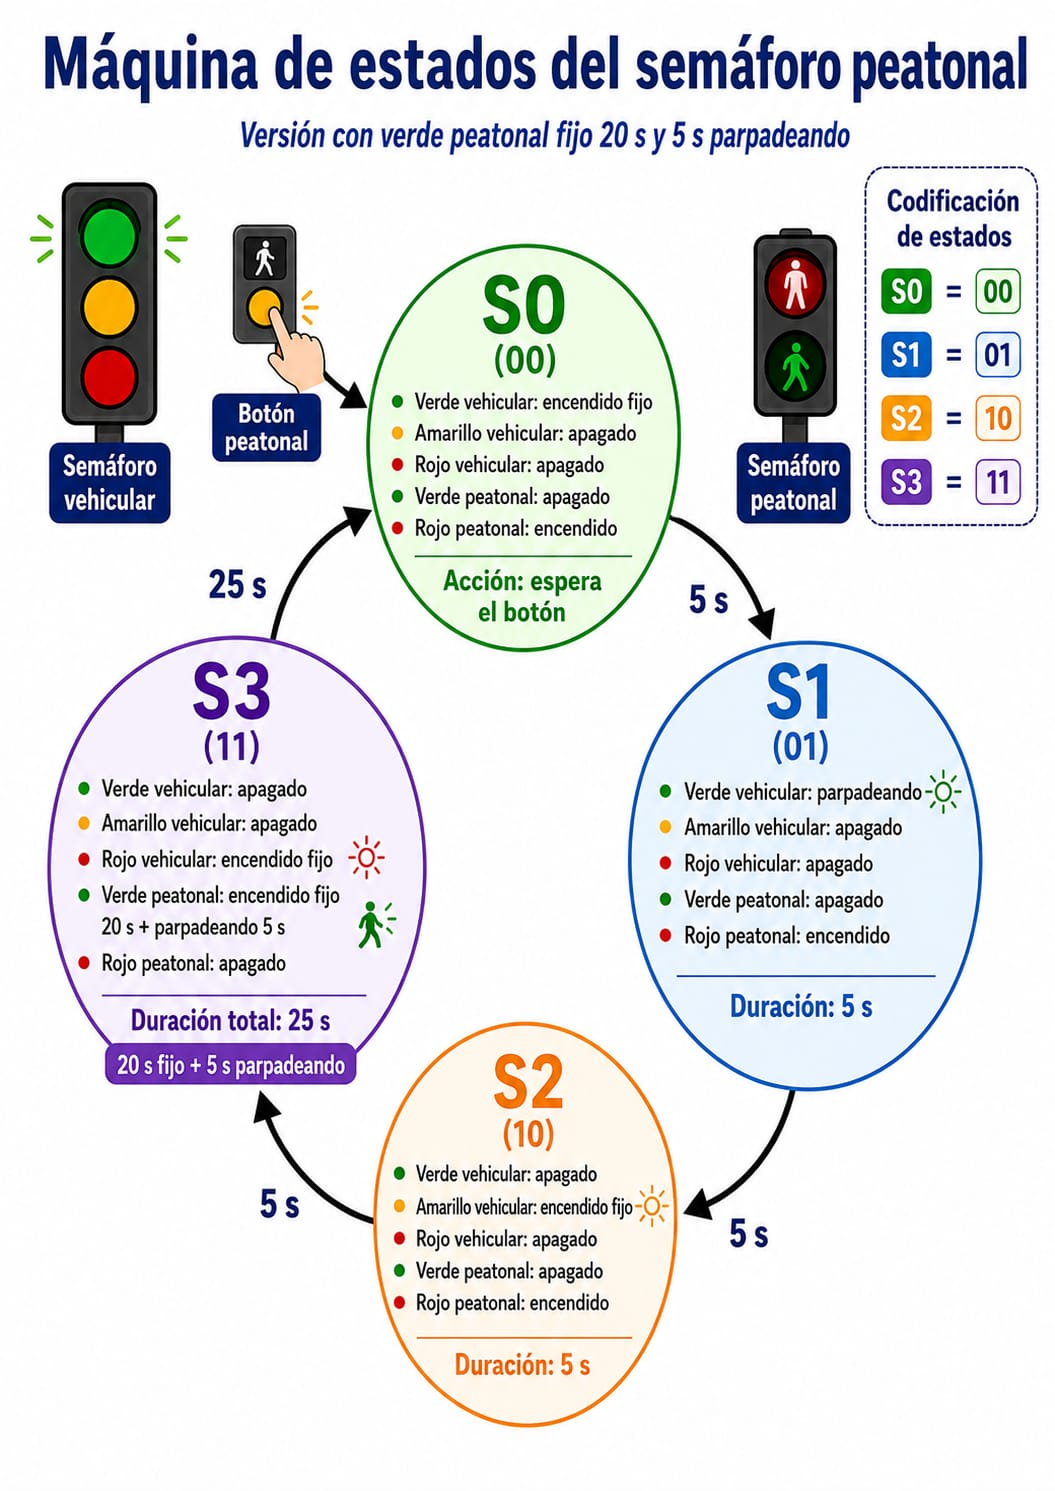
\includegraphics[width=1\textwidth]{Diagrama_de_FSM.jpeg}
		\caption{Diagrama del flujo de la máquina de estado.}
		\label{fsm1}
	\end{figure}

El estado inicial, $S_0$ ($00$), corresponde al estado de reposo del sistema. En esta condición permanecen encendidos el semáforo vehicular en verde y el semáforo peatonal en rojo, indicando el paso exclusivo para los vehículos. El sistema permanece en este estado hasta que se detecta la pulsación del botón peatonal, momento en el cual se realiza la transición hacia el estado $S_1$.\\

El estado $S_1$ ($01$) tiene una duración de 5 segundos. Durante este intervalo el semáforo vehicular verde comienza a parpadear, advirtiendo a los conductores del cambio de estado. Finalizado este tiempo, la máquina de estados avanza automáticamente al estado $S_2$.\\

En el estado $S_2$ ($10$), el semáforo vehicular cambia a amarillo fijo durante otros 5 segundos. Esta etapa funciona como una transición entre el paso vehicular y el paso peatonal, permitiendo que los vehículos despejen la intersección antes de detenerse completamente.\\

Finalmente, el sistema entra al estado $S_3$ ($11$), el cual tiene una duración total de 25 segundos. En este estado se enciende el semáforo vehicular rojo y simultáneamente el semáforo peatonal verde, permitiendo el cruce seguro de los peatones. El tiempo restante para el cruce se muestra mediante los displays de siete segmentos. Durante los últimos 5 segundos de este estado, el LED verde peatonal comienza a parpadear para advertir que el tiempo de cruce está por finalizar. De forma simultánea, el sistema auditivo pasa de emitir pulsos lentos a pulsos rápidos con el fin de proporcionar una advertencia adicional. Una vez concluidos los 25 segundos, la máquina retorna automáticamente al estado de reposo $S_0$, reiniciando el ciclo de funcionamiento.\\

El control temporal de cada uno de los estados se realiza mediante un contador decimal CD4017, el cual recibe como entrada la señal de reloj proveniente del temporizador 555. Las diferentes salidas del contador son empleadas por la lógica combinacional para determinar la duración de cada estado y generar las transiciones correspondientes. Adicionalmente, la lógica combinacional utiliza las variables de estado almacenadas en los flip-flops para controlar el encendido de los LED indicadores, el funcionamiento de los displays de siete segmentos y la generación de las señales de control del sistema sonoro.\\

Los LED correspondientes a los semáforos son controlados mediante transistores BJT utilizados como interruptores electrónicos, permitiendo manejar la corriente requerida por cada indicador sin sobrecargar las salidas de la lógica digital. Cada LED cuenta con su respectiva resistencia limitadora de corriente y es alimentado a partir de la fuente de 5 V del sistema.\\

\subsection{Diagrama del circuito}

	\begin{figure}[H]
		\centering
		
\includegraphics[width=0.7\textwidth]{Diagrama_Multisim_FSM.jpg}
		\caption{Diagrama del circuito de la FSM con los leds en el software Multisim.}
		\label{fsm1}
	\end{figure}
	
\subsection{Justificación de diseño}

La implementación de la máquina de estados se realizó utilizando un clock debido a que este tipo de arquitectura permite controlar de forma ordenada la secuencia de eventos del semáforo, garantizando que cada transición ocurra únicamente cuando se cumplen las condiciones establecidas y evitando cambios indeseados en las salidas.

\begin{itemize}

    \item Temporizador 555: Se seleccionó un temporizador 555 configurado en modo astable para generar la señal de reloj del sistema por su precisión para controlar las transiciones temporizadas de la máquina de estados.

    \item Flip-flops JK CD4027: Se emplearon dos flip-flops JK debido a que con ellos es posible almacenar los dos bits que representan los cuatro estados de funcionamiento del sistema.

    \item Lógica combinacional: La lógica combinacional se diseñó para generar tanto las ecuaciones de próximo estado como las señales de salida respectivas de cada estado. Esta implementación permite controlar de manera simultánea el encendido de los semáforos vehiculares y peatonales, la activación del sistema sonoro y las señales de control requeridas por el resto del circuito.

    \item Contador CD4017: Se utilizó un contador decimal CD4017 para controlar la duración de cada estado mediante la generación de pulsos de reloj provenientes del temporizador 555. Las salidas del contador se emplean para habilitar las transiciones entre estados y sincronizar el funcionamiento de los displays de siete segmentos.

    \item LEDs transistorizados: Aunque la lógica CMOS es capaz de suministrar corriente limitada, se utilizaron transistores BJT como interruptores para accionar los LED de los semáforos. Esto evita sobrecargar las salidas de los circuitos integrados y permite alimentar los indicadores directamente desde la fuente de 5V sin afectar el funcionamiento de la lógica digital.

\end{itemize}

\newpage

\section{\textbf{Display 7-Segmentos}}
\subsection{Descripción}
El módulo de display fue diseñado para implementar el conteo regresivo visual del sistema de semáforo vehicular y peatonal. Su función principal consiste en mostrar al usuario el tiempo restante disponible durante la habilitación del paso peatonal.\\

El sistema utiliza un temporizador 555 en configuración astable como generador de pulsos de reloj, encargado de producir la señal periódica que sincroniza el conteo. Esta señal es enviada a dos contadores BCD CD4510, uno destinado al manejo de las unidades y otro al de las decenas del conteo regresivo.\\

Las salidas BCD de cada contador son conectadas a decodificadores CD4511, los Las salidas BCD de cada contador son conectadas a decodificadores CD4511, los cuales convierten la información binaria en las señales necesarias para controlar los displays de 7 segmentos. Además, cada segmento incorpora una resistencia limitadora de corriente de 330\,$\Omega$ con el objetivo de proteger tanto los displays como los circuitos integrados.\\

El módulo fue configurado para iniciar el conteo en 20 segundos, disminuyendo progresivamente hasta llegar a 00, permitiendo visualizar el tiempo restante para el cruce peatonal. Además, se implementará una lógica de detección de cero mediante compuertas lógicas, de manera que cuando el sistema detecta simultáneamente 00 en decenas y unidades, el reloj queda bloqueado y el contador deja de disminuir, evitando conteos inválidos posteriores al cero.


\subsection{Diagrama del circuito}
	% Descomente y ajuste el nombre de la imagen:
	
	\begin{figure}[H]
		\centering
		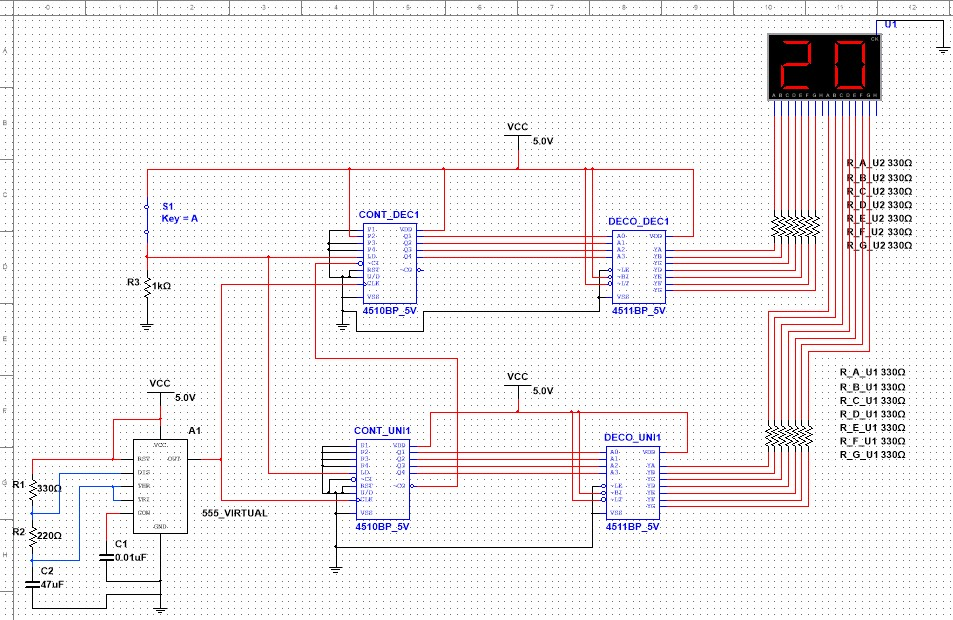
\includegraphics[width=0.9\textwidth]{Diagrama_Multisim_Display.jpg}
		\caption{Diagrama del circuito del Display de 7-segmentos en el software Multisim.}
		\label{diag_circuito_display}
	\end{figure}
		
	
\subsection{Justificación de diseño}
El diseño del módulo de display se desarrolló utilizando componentes digitales discretos debido a la necesidad de implementar un sistema de conteo regresivo confiable, visible y compatible con la lógica general del semáforo peatonal. Se seleccionaron contadores BCD CD4510 porque permiten realizar conteos descendentes de manera sencilla y facilitan la manipulación de valores decimales sin requerir lógica adicional compleja.\\

Asimismo, se emplearon decodificadores CD4511 debido a su compatibilidad directa con displays de 7 segmentos de cátodo común, reduciendo significativamente la cantidad de conexiones y simplificando la implementación física del sistema. Esto permite obtener una visualización clara del tiempo restante para el cruce peatonal.\\

La utilización del temporizador 555 como generador de reloj se debe a su facilidad de configuración, estabilidad y bajo costo, permitiendo generar pulsos periódicos necesarios para sincronizar el conteo del sistema. Además, las resistencias limitadoras fueron incorporadas para proteger los segmentos LED de sobrecorrientes y aumentar la confiabilidad del circuito.\\

Finalmente, de esta manera se puede verificar individualmente que este bloque sea funcional antes de integrar el sistema completo del semáforo.\\


\begin{figure}[H]
		\centering
		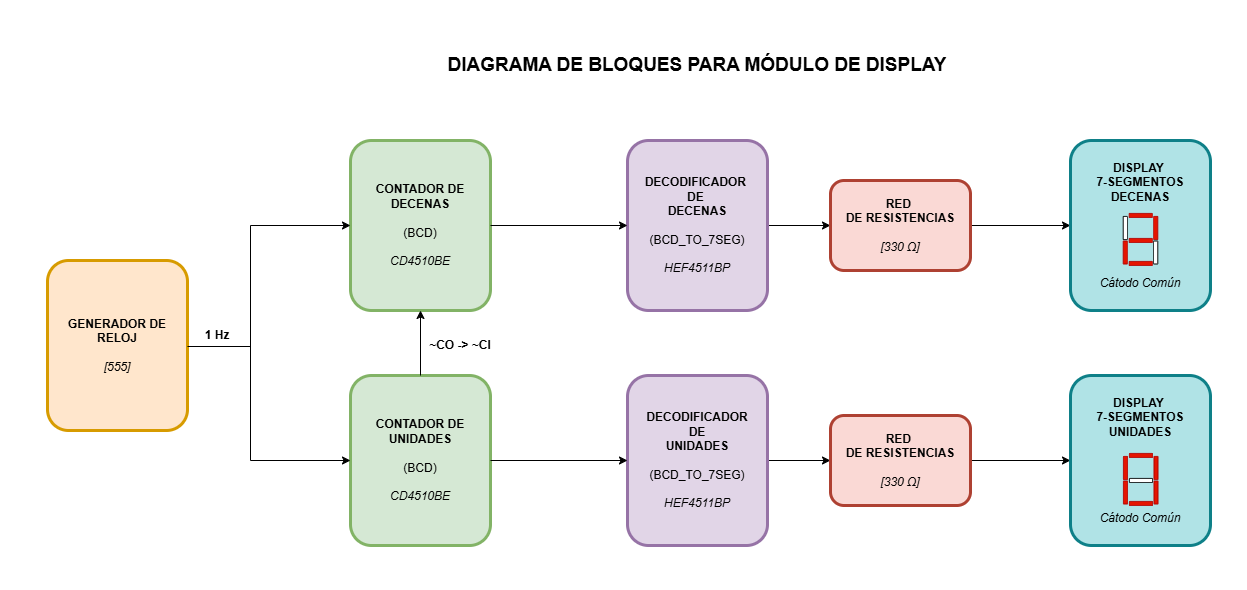
\includegraphics[width=1\textwidth]{Diagrama_de_bloques_Display.png}
		\caption{Diagrama de bloques para el Display.}
		\label{diag_bloq_display}
	\end{figure}
	
\newpage
	
\section{\textbf{Sistema de Señalización Auditiva}}

\subsection{Descripción}
Este sistema fue diseñado con el propósito de generar una señal auditiva para los peatones cuando este permitido cruzar la calle. Consiste en generar un sonido periódico cuando el semáforo peatonal se encuentre en verde y que este mismo se acelera una vez que falten cinco segundos para que se vuelva a poner en rojo. \\

Tomando en cuenta las especificaciones solicitadas cumpliendo únicamente con el uso de electrónica básica y sin ningún tipo de microcontroladores, se llego a la conclusión que la mejor forma de manejarlo era por medio de osciladores aestebles con circuitos integrados 555 que permiten ajustar la frecuencia deseada por medio de resistencias y capacitores.\\

Dado estos requerimientos se pude decir que el sistema completo se divide en los siguientes bloques funcionales principales:
\begin{enumerate}
    \item Generación del tono audible.
    \item Generación de la frecuencia de repetición lenta.
    \item Generación de la frecuencia de repetición rápida.
    \item Etapa de selección y amplificación de potencia.
\end{enumerate}

En cuanto al funcionamiento del circuito, todo inicia con la generación de tres señales cuadradas mediante temporizadores 555 configurados como osciladores astables. La primera corresponde al tono audible, con una frecuencia aproximada de 1\,kHz, seleccionada por encontrarse dentro del rango de mayor sensibilidad del oído humano y, por tanto, ser fácilmente perceptible. Adicionalmente, se generan dos señales de aproximadamente 1Hz y 2Hz, las cuales se emplean para producir las velocidades de repetición lenta y rápida del tono, respectivamente.\\

Posteriormente, la selección de la velocidad y la habilitación del sonido se realizan mediante un multiplexor (MUX). Este recibe como señales de control las salidas provenientes de la máquina de estados, específicamente las señales PEATONAL_ROJO y ULTIMOS_5_SEG. Dependiendo de la combinación de estas entradas, el multiplexor selecciona una de las tres posibles salidas: ausencia de sonido, repetición lenta (1Hz) o repetición rápida (2Hz). De esta manera, se concentra en un único bloque la lógica necesaria para determinar el comportamiento del sistema de audio según el estado del semáforo. La señal de salida habilitada por el multiplexor se combina finalmente mediante una compuerta AND con el tono audible de 1kHz.\\

Para la etapa de amplificación, dado que la lógica digital entrega una amplitud de 5V pero con una capacidad de corriente baja para el uso requerido, se implementa inicialmente un divisor de tensión para adaptar el nivel de entrada del amplificador. Posteriormente, la señal atraviesa un amplificador de dos etapas: una primera etapa de ganancia de voltaje basada en un transistor en configuración de emisor común y una segunda etapa de potencia tipo push-pull clase AB, ambas alimentadas con una fuente de 12V. Esta configuración proporciona tanto la ganancia de tensión como la capacidad de corriente necesarias para accionar el parlante de forma adecuada, garantizando un nivel de sonido adecuado para la aplicación.\\

\subsection{Diagrama del circuito}

	\begin{figure}[H]
		\centering
		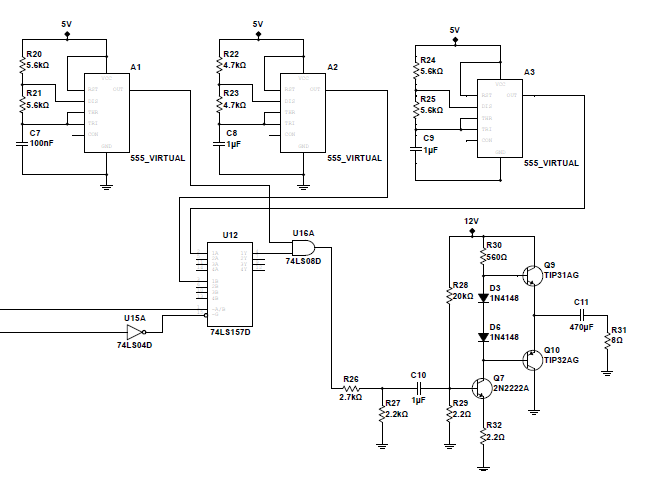
\includegraphics[width=0.7\textwidth]{circ audio.png}
		\caption{Diagrama del circuito de señalización auditiva.}
		\label{audio}
	\end{figure}

\subsection{Justificación de Diseño}
En esta sección se justifica la selección de los principales componentes utilizados en la implementación del circuito de generación y amplificación del tono audible.

\begin{itemize}

    \item Temporizadores 555: Se emplearon tres temporizadores 555 configurados en modo astable debido a su simplicidad, y estabilidad para generar señales cuadradas. Un primer temporizador produce el tono audible de aproximadamente 1kHz, mientras que los otros dos generan las frecuencias de repetición de 1Hz y 2Hz, correspondientes a las velocidades lenta y rápida requeridas. Además, estos circuitos integrados permiten ajustar fácilmente la frecuencia mediante la selección de resistencias y capacitores.

    \item Multiplexor: Se seleccionó un multiplexor como bloque de decisión debido a que simplifica considerablemente la lógica de selección de la señal de salida. A partir de las señales de control PEATONAL_ROJO y ULTIMOS_5_SEG, el MUX determina automáticamente si la salida debe permanecer deshabilitada o si debe haber una repetición lenta o rápida. Esta solución reduce la cantidad de compuertas lógicas necesarias.

    \item Compuerta AND: La salida del multiplexor se combina mediante una compuerta AND con la señal de 1kHz. De esta manera, el tono audible únicamente está presente cuando la señal de habilitación seleccionada por el MUX se encuentra activa.

    \item Divisor de tensión: Antes de la etapa de amplificación se implementó un divisor de tensión para adaptar el nivel de la señal proveniente de la lógica digital al valor requerido por la etapa amplificadora. Esto permite establecer un punto de operación adecuado para el transistor de entrada.

    \item Amplificador en emisor común: La primera etapa de amplificación corresponde a un amplificador de voltaje con transistor BJT en configuración de emisor común. Esta topología fue elegida por su elevada ganancia de voltaje, su facilidad de diseño.

    \item Etapa push-pull clase AB: Como etapa final se implementó un amplificador de potencia push-pull clase AB alimentado con 12V. Esta configuración proporciona la corriente necesaria para activar adecuadamente el parlante. Se debe tomar en cuenta que por la corriente manejada, se utilizaron transistores de potencia mucho mas robustos y con alta capacidad de disipación de calor.

    \item Parlante: Se utilizó un parlante para convertir la señal eléctrica amplificada en una señal sonora. La selección de un amplificador de potencia previo garantiza que el parlante reciba la corriente suficiente para producir un nivel de sonido adecuado para la aplicación.

\end{itemize}
\subsection{Gráficas}

\begin{figure}[H]
    \centering
    \begin{minipage}{0.45\textwidth}
        \centering
        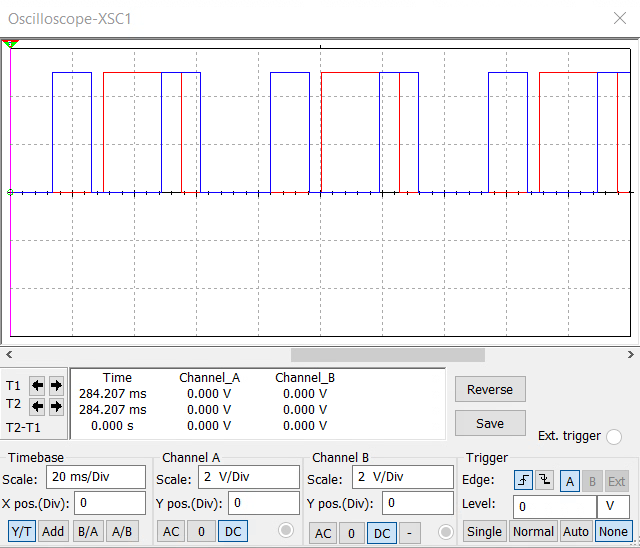
\includegraphics[width=0.9\textwidth]{osc velocidad.png}
		\caption{Señal de oscilación segun seleccion de velocidad.}
    \end{minipage}
    \hfill
    \begin{minipage}{0.45\textwidth}
        \centering
        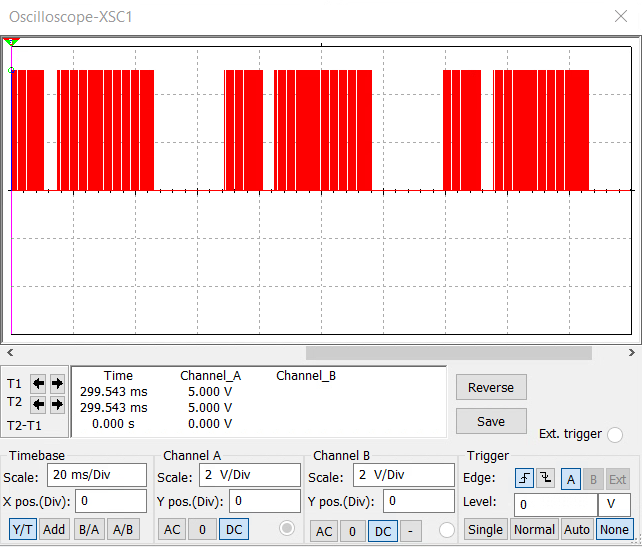
\includegraphics[width=0.9\textwidth]{salida lento.png}
		\caption{Ejemplo de tono de salida en modo lento.}
    \end{minipage}

\end{figure}

\newpage
	
\section{\textbf{Montaje físico y observaciones experimentales}}
Este apartado describe la construcción física del primer prototipo del circuito en protoboards. Contiene imágenes del montaje, los problemas experimentados durante el armado y los puntos clave observados durante las pruebas.
\subsection{Fotografias del montaje}
A continuación se muestran imágenes del montaje físico de cada circuito:

\begin{figure}[H]
	\centering
	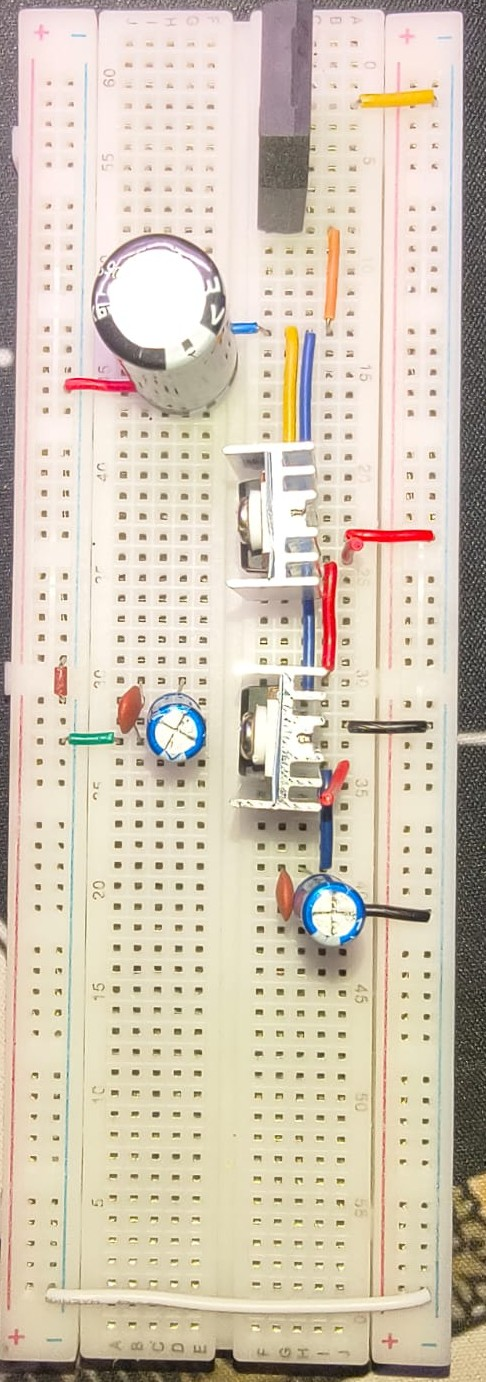
\includegraphics[width=0.3\textwidth,angle=90]{alimentacionfoto.jpeg}
	\caption{Circuito alimentacion en protoboard}
	\label{fig:alimentacionfoto}
\end{figure}

\subsection{Problemas encontrados}
Desde las primeras pruebas del prototipo completo, surgieron dificultades al integrar todos los módulos y ponerlos
a funcionar en conjunto.

\section{\textbf{Conclusiones}}
Se logró comprobar que es completamente viable diseñar un sistema de semáforo vehicular y peatonal complejo utilizando únicamente electrónica básica y componentes discretos, cumpliendo con las especificaciones de diseño sin depender de microcontroladores programables. Esto nos ayudó a entender mejor cómo coordinar la lógica digital con bloques de potencia y control en una aplicación del mundo real.
Se verificó que el circuito de potencia cumple con reducir y rectificar de manera segura los 120 $V_{rms}$ de la red eléctrica para entregar salidas fijas y reguladas de 5 V y 12 V. Durante el diseño, se evidenció que la correcta selección de los capacitores de filtro y desacople es vital para eliminar el rizado y absorber el ruido transitorio provocado por los constantes cambios de estado lógicos.	
	
\begin{thebibliography}{99}
\bibitem{Floyd}
T. L. Floyd, \textit{Dispositivos Electrónicos}, 8.a ed. México: Pearson Prentice Hall, 2008.

\bibitem{555video}
MADE IN COLOMBIA, ``Circuito integrado 555 explicación completa,'' YouTube, Dec. 16, 2017. [Online]. Available: \url{https://www.youtube.com/watch?v=n15R_n_TshA}

\bibitem{555delay}
``Cómo construir un circuito temporizador 555 con un retardo de apagado,'' Learning About Electronics. [Online]. Available: \url{https://www.learningaboutelectronics.com/Articulos/Circuito-temporizador-555-con-retardo-de-apagado.php}

\bibitem{CD4017video}
ElectronicaLED, ``Conexión y funcionamiento del circuito integrado CD4017,'' YouTube, Jun. 27, 2020. [Online]. Available: \url{https://www.youtube.com/watch?v=WflcnppydVY}

\bibitem{4017datasheet}
``IC 4017 Datasheet,'' ElecCircuit. [Online]. Available: \url{https://www.eleccircuit.com/ic-4017-datasheet/}

\bibitem{74192}
``74LS192 Decade Up/Down Counter With Clear Datasheet,'' Datasheet Hub. [Online]. Available: \url{https://www.datasheethub.com/74ls192-decade-up-down-counter-with-clear/}

\bibitem{74LS32}
``74LS32 Quad 2-Input OR Logic Gate IC Datasheet,'' Circuits DIY. [Online]. Available: \url{https://www.circuits-diy.com/74ls32-quad-2-input-or-logic-gate-ic-datasheet/}

\bibitem{74LS08}
``74LS08 Quad 2-Input AND Gate Datasheet,'' Datasheet Hub. [Online]. Available: \url{https://www.datasheethub.com/74ls08-quad-2-input-and-gate/}

\bibitem{displayvideo}
``Funcionamiento del display de 7 segmentos,'' YouTube. [Online]. Available: \url{https://www.youtube.com/watch?v=892DbbZ_GYM}

\bibitem{countervideo}
``Implementación de contadores digitales y displays,'' YouTube. [Online]. Available: \url{https://www.youtube.com/watch?v=PSDCvyHsHbk}

\bibitem{fsmvideo}
``Máquinas de estados y lógica secuencial,'' YouTube. [Online]. Available: \url{https://www.youtube.com/watch?v=8t-BtlKVZ7g}

\bibitem{fuentes}
J. Silva-Martínez and E. Sánchez-Sinencio, ``Diseño e implementación de fuentes de alimentación lineales reguladas para laboratorios de electrónica,'' \textit{Revista de Educación en Ingeniería Eléctrica}, vol. 14, no. 2, pp. 45--52, Jul. 2018.

\bibitem{Sadiku}
M. N. O. Sadiku and C. K. Alexander, \textit{Fundamentos de Circuitos Eléctricos}, 7.a ed. Ciudad de México, México: McGraw-Hill, 2021.

\bibitem{74LS14}
Renesas Technology Corp., ``HD74LS14 Hex Schmitt Trigger Inverters Datasheet,'' Rev. 3.00, Jul. 2005.

\bibitem{4511}
Philips Semiconductors, ``HEF4511B BCD to 7-Segment Latch/Decoder/Driver Datasheet,'' Jan. 1995.

\bibitem{555datasheet}
Texas Instruments, ``NA555, NE555, SA555, SE555 Precision Timers Datasheet,'' Rev. I, Sep. 2014.

\end{thebibliography}

\end{document}
